\documentclass[12pt]{article}

\usepackage{sbc-template}
\usepackage[T1]{fontenc}
\usepackage[utf8]{inputenc}
\usepackage[brazil]{babel}
\usepackage{amsmath}
\usepackage{amssymb}
\usepackage{booktabs}
\usepackage{tabularx}
\usepackage{multirow}
\usepackage{float}
\usepackage{xcolor}
\usepackage{enumitem}
\usepackage{array}
\usepackage{url}
\usepackage{hyperref}
\usepackage{graphicx}

\hypersetup{
  colorlinks=true,
  linkcolor=black,
  citecolor=black,
  urlcolor=blue
}

\newcolumntype{Y}{>{\raggedright\arraybackslash}X}
\newcommand{\todo}[1]{\textcolor{red}{[PREENCHER: #1]}}
\newcommand{\pavd}{PAVD}
\newcommand{\clip}{CLIP}
\newcommand{\sift}{SIFT}
\newcommand{\ssim}{SSIM}
\newcommand{\faiss}{FAISS}

\title{Protocolo Híbrido de Auditoria Visual para Localização, Verificação e Documentação de Imagens em Datasets de Treinamento}

\author{
  Pedro Garcia Ribas\inst{1}
}

\address{
  Instituto Federal de Minas Gerais -- Campus Sabará\\
  Bacharelado em Sistemas de Informação\\
  \email{pedro.garcia@estudante.ifmg.edu.br}
}

\begin{document}

\maketitle

\begin{abstract}
This work proposes the Visual Dataset Auditing Protocol (\pavd), a reproducible
experimental protocol for locating, verifying, rejecting, and documenting
potential visual correspondences between degraded query images and items in
galleries derived from web-scale datasets. The protocol separates global
retrieval, local geometric verification, open-set rejection, and technical
evidence reporting. A closed-set experiment with 500 JPEG images from the
English aesthetic subset of LAION-2B was measured on CPU using SSIM, SIFT with
Lowe's ratio test and RANSAC, and OpenAI CLIP ViT-B/32. The measured Top-1
accuracies were 88.6\%, 99.2\%, and 99.6\%, respectively. These values describe
only the tested convenience gallery and controlled degradation pipeline; they
are not properties of LAION, evidence of model training, or legal conclusions.
The expanded gallery, approximate vector indexing, hybrid reranking, and
open-set evaluation are specified as reproducible experimental blocks and
remain subject to measurement where results are not yet available.
\end{abstract}

\begin{resumo}
Este trabalho propõe o Protocolo de Auditoria Visual de Datasets (\pavd), um
protocolo experimental reproduzível para localizar, verificar, rejeitar e
documentar possíveis correspondências visuais entre imagens de consulta
degradadas e itens de galerias derivadas de datasets de larga escala. O
protocolo separa recuperação global, verificação geométrica local, rejeição em
conjunto aberto e produção de relatório de evidência técnica. Foi medido um
experimento em conjunto fechado com 500 imagens JPEG do recorte estético em
inglês do LAION-2B, em CPU, usando SSIM, SIFT com teste de razão de Lowe e
RANSAC, e CLIP OpenAI ViT-B/32. As acurácias Top-1 medidas foram,
respectivamente, 88,6\%, 99,2\% e 99,6\%. Esses valores descrevem somente a
galeria de conveniência e o pipeline de degradação controlada utilizados; não
são propriedades do LAION, evidência de treinamento de modelo ou conclusão
jurídica. A galeria expandida, o índice vetorial aproximado, o reranking
híbrido e a avaliação em conjunto aberto são especificados como blocos
experimentais reproduzíveis, permanecendo como \todo{resultados a medir} onde
não há dados disponíveis.
\end{resumo}

\section{Introdução}

Datasets web-scale de imagem e texto reúnem bilhões de pares coletados a partir
de páginas públicas. O LAION-5B, por exemplo, foi descrito como uma coleção de
aproximadamente 5,85 bilhões de pares imagem-texto \cite{schuhmann2022laion}.
Esse contexto torna relevante a construção de procedimentos capazes de
localizar itens potencialmente correspondentes a uma imagem de consulta sem
confundir correspondência visual com autoria, titularidade, licença, infração
ou participação efetiva no treinamento de qualquer modelo.

Uma imagem consultada raramente permanece idêntica ao arquivo originalmente
publicado. Redimensionamento, recorte, ruído e recompressão alteram os pixels,
mas podem preservar estruturas locais ou características semânticas. Técnicas
baseadas em comparação estrutural, descritores locais e embeddings
multimodais, portanto, respondem a aspectos diferentes do problema
\cite{wang2004ssim,lowe2004sift,radford2021clip}.

O trabalho propõe o \emph{Protocolo de Auditoria Visual de Datasets} (\pavd{}),
formulado como protocolo técnico experimental e não como norma jurídica. Seu
objetivo é organizar quatro operações: recuperação de candidatos,
verificação de correspondência, rejeição de consultas ausentes e
documentação de evidências computacionais. A formulação científica adotada é:

\begin{quote}
O trabalho propõe um protocolo experimental reproduzível para localização,
verificação, rejeição e documentação de potenciais correspondências visuais
entre imagens de consulta e itens de galerias derivadas de datasets
web-scale.
\end{quote}

O experimento já medido é de conjunto fechado: cada consulta é uma cópia
degradada de uma imagem que permanece na galeria de 500 itens. A expansão para
aproximadamente 100 mil imagens, a busca com \faiss{}, o reranking local e o
conjunto aberto são definidos neste documento, mas não recebem resultados
inventados.

\section{Objetivos}

\subsection{Objetivo geral}

Propor e documentar o \pavd{} como um protocolo experimental reproduzível para
auditoria visual de galerias derivadas de datasets de treinamento, separando
recuperação global, verificação local, rejeição de ausentes e registro de
evidências técnicas.

\subsection{Objetivos específicos}

\begin{itemize}[leftmargin=*]
  \item comparar \ssim{}, \sift{} com teste de razão de Lowe e RANSAC, e
  \clip{} ViT-B/32 em um conjunto fechado com degradação controlada;
  \item medir Top-1, custo de indexação e tempo de consulta no cenário
  experimental de 500 imagens;
  \item especificar a avaliação de recuperação Top-$K$, MRR, custo e memória
  em uma galeria expandida;
  \item avaliar, quando executado, o efeito de reranking local sobre
  candidatos recuperados por \clip{};
  \item definir uma política de rejeição de consultas ausentes com partições
  de calibração e teste;
  \item produzir relatórios por consulta contendo hashes, parâmetros,
  versões, candidatos, scores e evidências visuais;
  \item delimitar o que pode ser afirmado a partir de uma correspondência
  visual e o que exige revisão humana, perícia ou análise jurídica.
\end{itemize}

\section{Referencial Teórico}

\subsection{Auditoria de datasets e recuperação visual}

Auditar uma galeria visual envolve mais do que retornar um vizinho próximo.
É necessário preservar a identidade do item, registrar sua origem e distinguir
um resultado de recuperação de uma decisão sobre direitos. O \pavd{} adota,
assim, a rastreabilidade do item como parte da avaliação: cada imagem deve ser
associada a identificadores, URL de origem, hash, estado do download e
informações de processamento.

O LAION-5B foi construído a partir de dados disponíveis na web e seus itens
estão associados a metadados e URLs, não a uma garantia de armazenamento
permanente dos arquivos JPEG \cite{schuhmann2022laion}. Neste trabalho, os
JPEGs são arquivos obtidos localmente a partir de URLs do recorte de
metadados. O dataset experimental é exclusivamente
\texttt{laion/laion2B-en-aesthetic} \cite{laion2022aesthetic,laion2022dataset};
LAION-Art, Re-LAION e LAION-400M não são utilizados como galerias
experimentais.

\subsection{SSIM}

O índice de similaridade estrutural compara luminância, contraste e estrutura
em janelas correspondentes \cite{wang2004ssim}. Para duas janelas $x$ e $y$,
uma forma simplificada é:

\begin{equation}
\operatorname{SSIM}(x,y)=
\frac{(2\mu_x\mu_y+C_1)(2\sigma_{xy}+C_2)}
{(\mu_x^2+\mu_y^2+C_1)(\sigma_x^2+\sigma_y^2+C_2)},
\label{eq:ssim}
\end{equation}

em que $\mu_x$ e $\mu_y$ são médias, $\sigma_x^2$ e $\sigma_y^2$ são
variâncias, $\sigma_{xy}$ é a covariância e $C_1,C_2$ estabilizam o cálculo.
No experimento medido, as imagens foram convertidas para tons de cinza,
normalizadas para a faixa $[0,1]$ e redimensionadas para $128\times128$.
No cenário de 500 imagens, a busca compara cada consulta com toda a galeria.

\subsection{SIFT, teste de Lowe e RANSAC}

O SIFT identifica pontos de interesse e descritores locais robustos a mudanças
de escala e rotação \cite{lowe2004sift}. O teste de razão de Lowe reduz
correspondências ambíguas, comparando a distância do vizinho mais próximo com
a do segundo vizinho. O RANSAC pode então estimar uma transformação geométrica
e separar correspondências consistentes de outliers \cite{fischler1981ransac}.

Descritores locais podem ser úteis quando o recorte desloca o conteúdo, mas a
quantidade de pontos depende da textura e da estrutura da imagem. Em
particular, itens com áreas planas, logotipos ou vetores podem apresentar
poucos keypoints. Essa observação deve ser analisada condicionalmente à
amostra, e não transformada em uma afirmação universal sobre uma categoria.

\subsection{CLIP e busca vetorial}

O CLIP aprende representações alinhadas entre imagens e linguagem a partir de
supervisão natural em larga escala \cite{radford2021clip}. Neste trabalho, o
modelo \texttt{openai/clip-vit-base-patch32} produz vetores de dimensão 512.
Após normalização L2, o produto interno entre vetores coincide com a
similaridade do cosseno:

\begin{equation}
\operatorname{cos}(q,g)=
\frac{\mathbf{e}_q\cdot\mathbf{e}_g}
{\lVert\mathbf{e}_q\rVert_2\lVert\mathbf{e}_g\rVert_2}.
\label{eq:cosine}
\end{equation}

Para vetores normalizados, a expressão é simplesmente
$\mathbf{e}_q\cdot\mathbf{e}_g$. Em uma galeria maior, bibliotecas como
\faiss{} permitem buscar vizinhos em espaços vetoriais com índices exatos ou
aproximados \cite{johnson2019faiss}.

\subsection{Detecção de cópias e representações visuais}

Descritores orientados à detecção de cópias, como SSCD, constituem uma
possibilidade exploratória distinta da representação multimodal do CLIP
\cite{pizzi2022sscd}. DINOv2 representa uma alternativa de representação
visual auto-supervisionada \cite{oquab2024dinov2}. Esses métodos não
substituem os três métodos oficiais da comparação e só devem ser incluídos
com resultados se forem executados nas 500 consultas.

Trabalhos sobre replicação de dados, deduplicação, detecção de infração
autoral e extração de dados de modelos de difusão motivam a necessidade de
cautela na interpretação dos resultados
\cite{somepalli2023diffusion,carlini2023extracting,webster2023deduplication,
huang2025mcid}.
Eles não autorizam inferir, a partir da presença de um item em uma galeria,
que um modelo específico o tenha utilizado ou memorizado.

\subsection{Recuperação global--local}

Uma arquitetura em duas etapas pode usar uma representação global para
recuperar candidatos e uma verificação local para confirmar consistência
geométrica. O fluxo estudado pelo \pavd{} é:

\begin{center}
\textit{consulta $\rightarrow$ CLIP ViT-B/32 $\rightarrow$ FAISS Top-50
$\rightarrow$ SIFT + Lowe + RANSAC $\rightarrow$ decisão técnica}.
\end{center}

Essa composição é tratada como arquitetura experimental a ser avaliada, não
como invenção do trabalho.

\section{Protocolo de Auditoria Visual de Datasets}

\subsection{Visão geral}

O \pavd{} organiza o processo em quatro camadas:

\begin{enumerate}[leftmargin=*]
  \item \textbf{localização global}: recuperação de candidatos por \clip{} e,
  em pequena escala, comparação exaustiva;
  \item \textbf{verificação local}: análise de keypoints, matches, inliers,
  homografia e erro de reprojeção;
  \item \textbf{rejeição}: decisão de presença ou ausência com limiares
  calibrados em uma partição independente;
  \item \textbf{documentação}: geração de evidência técnica reproduzível,
  sem convertê-la automaticamente em prova jurídica.
\end{enumerate}

\begin{table}[H]
\centering
\caption{Componentes do \pavd{}.}
\label{tab:componentes}
\begin{tabularx}{\linewidth}{p{0.23\linewidth}Y Y}
\toprule
\textbf{Componente} & \textbf{Função} & \textbf{Saída principal}\\
\midrule
Galeria rastreável & Preservar identidade e origem dos itens & Metadados,
hashes e estados\\
Degradação controlada & Gerar consultas reproduzíveis & Consulta e parâmetros\\
Recuperação global & Ordenar candidatos em escala & Top-$K$ e scores\\
Verificação local & Testar consistência geométrica & Matches, inliers e erro\\
Rejeição aberta & Evitar atribuição de ausentes & Decisão e limiar\\
Relatório & Permitir revisão e repetição & Evidência por consulta\\
\bottomrule
\end{tabularx}
\end{table}

\begin{table}[H]
\centering
\caption{Afirmações permitidas e não permitidas.}
\label{tab:afirmacoes}
\begin{tabularx}{\linewidth}{Y Y}
\toprule
\textbf{Permitido} & \textbf{Não permitido}\\
\midrule
Há correspondência visual entre a consulta e um item da galeria experimental. &
O modelo treinou com a obra identificada.\\
O método recuperou o mesmo item-fonte sob a degradação testada. &
A presença prova scraping ilícito, infração ou ausência de licença.\\
O resultado constitui evidência técnica reproduzível para auditoria, revisão
humana e eventual análise especializada. &
O resultado constitui prova jurídica conclusiva.\\
O desempenho foi observado nesta galeria e configuração. &
O desempenho é propriedade geral do LAION ou de qualquer dataset.\\
\bottomrule
\end{tabularx}
\end{table}

\section{Metodologia}

\subsection{Dataset e galerias}

O dataset utilizado é exclusivamente \texttt{laion/laion2B-en-aesthetic},
considerando itens em inglês e o recorte estético superior a 7. A galeria
oficial medida contém 500 JPEGs válidos, obtidos a partir das primeiras URLs
que responderam no streaming. Trata-se de uma amostra de conveniência, não de
sorteio nem de amostra estatisticamente representativa.

Os arquivos foram nomeados de \texttt{laion\_001.jpg} a
\texttt{laion\_500.jpg}. O downloader aplicou timeout de 3 segundos, limite de
corpo de 20 MB e descartou respostas 404, timeouts, corpos vazios e arquivos
não reconhecidos pelo Pillow. A galeria expandida prevista contém
aproximadamente 100 mil imagens, incluindo obrigatoriamente as 500 fontes
oficiais e 100 itens adicionais URL-only do mesmo recorte. A expansão não
é uma amostra aleatória.

\begin{table}[H]
\centering
\caption{Metadados mínimos por item da galeria.}
\label{tab:metadados}
\begin{tabularx}{\linewidth}{p{0.31\linewidth}Y}
\toprule
\textbf{Campo} & \textbf{Finalidade}\\
\midrule
\texttt{gallery\_id} & Identificador do item na galeria\\
\texttt{source\_id} & Identificador do item no recorte de origem\\
\texttt{source\_url} & URL associada ao metadado\\
\texttt{download\_timestamp} & Data, hora e fuso da coleta\\
\texttt{sha256} & Integridade do arquivo local\\
\texttt{mime\_type}, \texttt{width}, \texttt{height} & Caracterização técnica\\
\texttt{download\_status} & Sucesso, falha ou motivo de descarte\\
\texttt{visual\_category} & Estrato operacional de análise\\
\texttt{visual\_category\_confidence} & Confiança da classificação, quando houver\\
Redirecionamento e duplicidade & Rastreabilidade de mudanças e deduplicação\\
Motivo de exclusão & Registro explícito de itens removidos\\
\bottomrule
\end{tabularx}
\end{table}

\subsection{Categorias visuais}

As categorias operacionais são fotografia, pintura digital, arte vetorial,
logo, colagem e ambígua ou mista. Uma classificação inicial pode usar
\clip{} zero-shot, mas não deve ser tratada como verdade ontológica. Uma
subamostra estratificada deve ser revisada manualmente, registrando a
quantidade revisada por categoria.

\begin{table}[H]
\centering
\caption{Distribuição de categorias visuais.}
\label{tab:categorias}
\begin{tabularx}{\linewidth}{Y r r Y}
\toprule
\textbf{Categoria} & \textbf{Quantidade} & \textbf{Revisada} & \textbf{Critério}\\
\midrule
Fotografia & \todo{n} & \todo{n} & \todo{descrição}\\
Pintura digital & \todo{n} & \todo{n} & \todo{descrição}\\
Arte vetorial & \todo{n} & \todo{n} & \todo{descrição}\\
Logo & \todo{n} & \todo{n} & \todo{descrição}\\
Colagem & \todo{n} & \todo{n} & \todo{descrição}\\
Ambígua ou mista & \todo{n} & \todo{n} & \todo{descrição}\\
\bottomrule
\end{tabularx}
\end{table}

\subsection{Pipeline de degradação}

Cada uma das 500 consultas oficiais é produzida a partir do JPEG local
correspondente, preservando o mesmo identificador. A ordem fixa é escala
0,80, crop de 5\% de cada borda, ruído gaussiano com $\sigma=8$ e compressão
JPEG com qualidade 35.

\begin{table}[H]
\centering
\caption{Pipeline de degradação das consultas.}
\label{tab:degradacao}
\begin{tabularx}{\linewidth}{p{0.24\linewidth}Y}
\toprule
\textbf{Etapa} & \textbf{Configuração}\\
\midrule
Escala & Fator 0,80; interpolação por área (\texttt{INTER\_AREA})\\
Crop & 5\% de cada borda; preservar somente se restarem pelo menos 16 pixels\\
Ruído & Gaussiano, média 0, desvio-padrão 8, com valores limitados a 0--255\\
JPEG & Qualidade 35\\
Semente & \texttt{zlib.crc32} derivado do identificador da imagem\\
\bottomrule
\end{tabularx}
\end{table}

Para reprodutibilidade completa, devem ser registrados a resolução após a
escala, coordenadas do crop, espaço de cor, faixa do ruído, biblioteca e
versão da compressão, subsampling JPEG, orientação EXIF, transparência e
política de conversão de cores. As imagens adicionais da galeria expandida
não são adulteradas.

\subsection{Métodos avaliados}

\subsubsection{SSIM}

No Bloco A, cada consulta é comparada com os 500 itens após conversão para
cinza e redimensionamento para $128\times128$. O maior SSIM define o Top-1.
Essa comparação é um baseline pareado e não é executada exaustivamente sobre
100 mil itens como experimento oficial. A complexidade aproximada é:

\begin{equation}
T_{\ssim}=O(Q\cdot N\cdot H\cdot W),
\label{eq:complexidade-ssim}
\end{equation}

em que $Q$ é o número de consultas, $N$ o tamanho da galeria e $H,W$ as
dimensões usadas na comparação.

\subsubsection{SIFT, Lowe e RANSAC}

São extraídos keypoints e descritores SIFT. O teste de razão de Lowe usa
limiar 0,75. No procedimento medido, descritores da galeria são colocados em
um \texttt{FlannBasedMatcher} com KD-tree, cinco árvores e
\texttt{checks=50}; os vizinhos aceitos votam na imagem de origem.

No protocolo expandido, devem ser registrados keypoints, matches, inliers,
razão de inliers, transformação estimada e erro de reprojeção. Consultas sem
keypoints, matches válidos ou homografia devem ser contabilizadas
explicitamente. Em uma galeria de 100 mil, \sift{} não deve ser chamado de
busca global quando executado apenas nos candidatos Top-50 do \clip{}; nesse
caso, ele é reranker ou verificador local.

\subsubsection{CLIP ViT-B/32}

Os embeddings são normalizados em norma L2 e comparados por produto interno.
No Bloco A, a busca é exata contra a matriz da galeria. No Bloco B, deve ser
medido um índice \faiss{} com tipo, parâmetros, dimensão, precisão, memória,
tempo de construção e tempo de consulta registrados. Uma amostra deve
comparar o ranking aproximado com o ranking exato.

\begin{table}[H]
\centering
\caption{Configuração experimental e parâmetros reproduzíveis.}
\label{tab:parametros}
\begin{tabularx}{\linewidth}{p{0.34\linewidth}Y}
\toprule
\textbf{Parâmetro} & \textbf{Valor}\\
\midrule
Modelo CLIP & \texttt{openai/clip-vit-base-patch32}\\
Dimensão do embedding & 512\\
Normalização & Norma L2; produto interno como cosseno\\
SIFT & \texttt{SIFT\_create(nfeatures=500)}\\
Razão de Lowe & 0,75\\
FLANN & KD-tree, cinco árvores, \texttt{checks=50}\\
SSIM & Cinza, float32 em $[0,1]$, $128\times128$, \texttt{data\_range=1}\\
FAISS & \todo{tipo e parâmetros do índice}\\
Hardware & CPU AMD64; sem GPU\\
Software & Python 3.13.4; OpenCV 5.0.0; scikit-image 0.26.0;
Transformers 5.17.0; PyTorch 2.14.0+cpu\\
\bottomrule
\end{tabularx}
\end{table}

\subsection{Blocos experimentais}

\begin{table}[H]
\centering
\caption{Blocos experimentais do \pavd{}.}
\label{tab:blocos}
\begin{tabularx}{\linewidth}{p{0.15\linewidth}p{0.26\linewidth}Y}
\toprule
\textbf{Bloco} & \textbf{Escopo} & \textbf{Medições}\\
\midrule
A & Conjunto fechado, $N=500$ & Top-1 e tempo de SSIM, SIFT e CLIP\\
B & Galeria expandida, $N\approx100.000$ & Top-$K$, MRR, ranks, memória,
indexação, busca e ANN Recall\\
C & Recuperação em duas etapas & Comparação de políticas de reranking local\\
D & Conjunto aberto & Presença, rejeição e falsa atribuição\\
\bottomrule
\end{tabularx}
\end{table}

\subsubsection{Bloco A: conjunto fechado}

O original está sempre presente. O acerto exige recuperar o mesmo
\texttt{gallery\_id} e o mesmo item-fonte que originou a consulta. Indexação e
carregamento são separados do tempo de consulta.

\begin{table}[H]
\centering
\caption{Resultados preliminares oficiais do Bloco A, medidos em 28 de setembro de 2026.}
\label{tab:resultados-a}
\begin{tabularx}{\linewidth}{Y r r r r}
\toprule
\textbf{Método} & \textbf{Acertos} & \textbf{Top-1} & \textbf{Indexação (s)}
& \textbf{Busca média (s)}\\
\midrule
SSIM & 443/500 & 88,6\% & 1,09 & 0,3507\\
SIFT + Lowe + RANSAC & 496/500 & 99,2\% & 21,56 & 0,0383\\
CLIP ViT-B/32 & 498/500 & 99,6\% & 43,04 & 0,0564\\
\bottomrule
\end{tabularx}
\end{table}

Esses valores são resultados da configuração local, em CPU AMD64 sem GPU,
com Python 3.13.4 e as versões registradas na Tabela~\ref{tab:parametros}.
Não são propriedades gerais do LAION. O CLIP apresentou o maior número de
acertos na galeria avaliada; o SIFT apresentou o menor tempo médio de busca;
o SSIM foi afetado pela comparação posicional após o crop. Essas leituras são
condicionadas ao pipeline fixo e não constituem superioridade universal.

\begin{table}[H]
\centering
\caption{Desempenho por categoria visual no Bloco A.}
\label{tab:categorias-a}
\begin{tabularx}{\linewidth}{Y r r r r r r}
\toprule
\textbf{Categoria} & \textbf{n} & \multicolumn{2}{c}{\textbf{SSIM}} &
\multicolumn{2}{c}{\textbf{SIFT}} & \textbf{CLIP}\\
\cmidrule(lr){3-4}\cmidrule(lr){5-6}
 & & \textbf{Top-1} & \textbf{s} & \textbf{Top-1} & \textbf{s} & \textbf{Top-1 / s}\\
\midrule
Fotografia & \todo{n} & \todo{\%} & \todo{s} & \todo{\%} & \todo{s} & \todo{\% / s}\\
Pintura digital & \todo{n} & \todo{\%} & \todo{s} & \todo{\%} & \todo{s} & \todo{\% / s}\\
Arte vetorial & \todo{n} & \todo{\%} & \todo{s} & \todo{s} & \todo{s} & \todo{\% / s}\\
Logo & \todo{n} & \todo{\%} & \todo{s} & \todo{\%} & \todo{s} & \todo{\% / s}\\
Colagem & \todo{n} & \todo{\%} & \todo{s} & \todo{\%} & \todo{s} & \todo{\% / s}\\
Ambígua ou mista & \todo{n} & \todo{\%} & \todo{s} & \todo{\%} & \todo{s} & \todo{\% / s}\\
\bottomrule
\end{tabularx}
\end{table}

\begin{table}[H]
\centering
\caption{Diagnóstico operacional do SIFT por categoria.}
\label{tab:sift-diagnostico}
\begin{tabularx}{\linewidth}{Y r r r r}
\toprule
\textbf{Categoria} & \textbf{Mediana de keypoints} & \textbf{Matches} &
\textbf{Inliers} & \textbf{Sem correspondência válida}\\
\midrule
Fotografia & \todo{valor} & \todo{valor} & \todo{valor} & \todo{\%}\\
Pintura digital & \todo{valor} & \todo{valor} & \todo{valor} & \todo{\%}\\
Arte vetorial & \todo{valor} & \todo{valor} & \todo{valor} & \todo{\%}\\
Logo & \todo{valor} & \todo{valor} & \todo{valor} & \todo{\%}\\
Colagem & \todo{valor} & \todo{valor} & \todo{valor} & \todo{\%}\\
Ambígua ou mista & \todo{valor} & \todo{valor} & \todo{valor} & \todo{\%}\\
\bottomrule
\end{tabularx}
\end{table}

\subsubsection{Bloco B: galeria expandida}

O Bloco B utiliza as mesmas 500 consultas e mantém suas fontes na galeria de
aproximadamente 100 mil imagens. O \clip{} com \faiss{} é o mecanismo de
recuperação global. Devem ser medidos Top-1, Recall@5, Recall@12, Recall@50,
MRR, mediana e percentil 95 do rank, tempos de embedding, busca e reranking,
memória e construção do índice.

\begin{equation}
\operatorname{Recall@K}=
\frac{1}{Q}\sum_{q=1}^{Q}
\mathbb{1}\{\operatorname{rank}(q)\leq K\}.
\label{eq:recall}
\end{equation}

\begin{equation}
\operatorname{MRR}=
\frac{1}{Q}\sum_{q=1}^{Q}\frac{1}{\operatorname{rank}(q)}.
\label{eq:mrr}
\end{equation}

Recall@12 é adotado por corresponder ao número de itens exibidos na grade da
interface. Recall@50 representa o orçamento de candidatos para SIFT+RANSAC.
Para separar a perda causada pelo índice aproximado da limitação do embedding,
define-se:

\begin{equation}
\operatorname{ANN\ Recall@K}=
\frac{\#\{q:\text{fonte verdadeira de }q\text{ aparece no Top-}K
\text{ do FAISS}\}}{Q}.
\label{eq:ann-recall}
\end{equation}

\begin{table}[H]
\centering
\caption{Qualidade de recuperação no Bloco B.}
\label{tab:qualidade-b}
\begin{tabularx}{\linewidth}{Y r r r r r r}
\toprule
\textbf{Método} & \textbf{Top-1} & \textbf{R@5} & \textbf{R@12} &
\textbf{R@50} & \textbf{MRR} & \textbf{P95 rank}\\
\midrule
CLIP + FAISS & \todo{\%} & \todo{\%} & \todo{\%} & \todo{\%} &
\todo{valor} & \todo{valor}\\
CLIP exato (amostra) & \todo{\%} & \todo{\%} & \todo{\%} & \todo{\%} &
\todo{valor} & \todo{valor}\\
\bottomrule
\end{tabularx}
\end{table}

\begin{table}[H]
\centering
\caption{Custo e configuração do índice no Bloco B.}
\label{tab:custo-b}
\begin{tabularx}{\linewidth}{Y Y}
\toprule
\textbf{Medida} & \textbf{Resultado}\\
\midrule
Tipo e parâmetros do índice & \todo{preencher}\\
Dimensão e precisão & 512; \todo{precisão}\\
Tempo de construção & \todo{preencher}\\
Tempo de embedding por consulta & \todo{preencher}\\
Tempo de busca & \todo{preencher}\\
Tempo de reranking & \todo{preencher}\\
Memória do índice & \todo{preencher}\\
ANN Recall@50 & \todo{preencher}\\
\bottomrule
\end{tabularx}
\end{table}

\subsubsection{Bloco C: recuperação em duas etapas}

São comparadas três políticas: (1) \clip{}+\faiss{} sem reranking; (2)
\clip{}+\faiss{} Top-50 seguido de SIFT+RANSAC para todas as consultas; e
(3) o mesmo reranking condicionado à categoria visual. A política
condicionada só pode ser considerada vantajosa se reduzir custo ou verificações
sem perda relevante de Top-1, MRR ou aumento de FAR. Caso a categoria seja
definida por zero-shot do próprio CLIP, a circularidade e a limitação devem
ser declaradas.

\begin{table}[H]
\centering
\caption{Ablação do pipeline híbrido no Bloco C.}
\label{tab:ablacao-c}
\begin{tabularx}{\linewidth}{Y r r r r Y}
\toprule
\textbf{Política} & \textbf{Top-1} & \textbf{MRR} & \textbf{FAR} &
\textbf{Tempo} & \textbf{Interpretação}\\
\midrule
CLIP + FAISS & \todo{\%} & \todo{valor} & \todo{\%} & \todo{s} &
\todo{preencher}\\
Top-50 + SIFT para todas & \todo{\%} & \todo{valor} & \todo{\%} & \todo{s} &
\todo{preencher}\\
Top-50 + SIFT por categoria & \todo{\%} & \todo{valor} & \todo{\%} & \todo{s} &
\todo{preencher}\\
\bottomrule
\end{tabularx}
\end{table}

\subsubsection{Bloco D: conjunto aberto}

O conjunto aberto inclui consultas cuja fonte não está na galeria. A regra
preliminar é:

\begin{equation}
\operatorname{Presente}(q)=
\begin{cases}
1,&s_1\geq0{,}82\ \lor\
(s_1\geq0{,}75\land s_1-s_2\geq0{,}10),\\
0,&\text{caso contrário},
\end{cases}
\label{eq:presenca}
\end{equation}

em que $s_1$ e $s_2$ são, respectivamente, os dois maiores scores CLIP.
Como dado preliminar, a mediana do score do par verdadeiro foi 0,915. No
exemplo isolado \texttt{fora.jpg}, o score foi 0,773 e a margem foi 0,014,
resultando em rejeição. Esse exemplo não é uma avaliação completa.

Os limiares são específicos da galeria, do encoder, do pipeline e da
distribuição de negativos. A calibração deve usar uma partição separada da
partição de teste, com negativos aleatórios, semanticamente próximos e
visualmente próximos da mesma categoria, porém ausentes da galeria.

\begin{equation}
\operatorname{FAR}=
\frac{\text{consultas ausentes aceitas como presentes}}
{\text{total de consultas ausentes}}.
\label{eq:far}
\end{equation}

\begin{table}[H]
\centering
\caption{Métricas previstas para o conjunto aberto.}
\label{tab:aberto}
\begin{tabularx}{\linewidth}{Y Y}
\toprule
\textbf{Métrica} & \textbf{Resultado}\\
\midrule
TPR de presença & \todo{preencher após partição de teste}\\
FAR & \todo{preencher após partição de teste}\\
Precisão dos aceitos & \todo{preencher}\\
Taxa de rejeição correta & \todo{preencher}\\
AUROC (opcional) & \todo{preencher}\\
FPR95 (opcional) & \todo{preencher}\\
\bottomrule
\end{tabularx}
\end{table}

\subsection{Relatório de evidência técnica}

O relatório por consulta é uma entrega do protocolo. Ele deve conter:

\begin{itemize}[leftmargin=*]
  \item \texttt{query\_id}, \texttt{gallery\_id}, \texttt{source\_id}, URL e
  data, hora e fuso da coleta;
  \item SHA-256 da consulta e do candidato, versão do código, sistema
  operacional, hardware e versões de Python, OpenCV, PyTorch, \faiss{} e
  CLIP/OpenCLIP;
  \item parâmetros de \ssim{}, \sift{}, razão de Lowe, RANSAC e \faiss{};
  \item Top-50, scores de cosseno, rank da fonte verdadeira e margem
  Top-1 menos Top-2;
  \item número de keypoints, matches, inliers, homografia e erro de
  reprojeção, quando estimados;
  \item decisão técnica: aceito tecnicamente, encaminhado para revisão ou
  rejeitado, acompanhada de justificativa;
  \item evidência visual da consulta, candidato, correspondências de
  keypoints e região geométrica compatível.
\end{itemize}

O relatório deve ser descrito como ``evidência técnica reproduzível para
auditoria, revisão humana e eventual análise especializada''. Não deve ser
descrito como prova jurídica conclusiva.

\section{Resultados e Discussão}

\subsection{Resultados preliminares do Bloco A}

Na amostra fechada de 500 imagens, o \clip{} identificou o item-fonte em
498 consultas (99,6\%), o \sift{} em 496 (99,2\%) e o \ssim{} em 443 (88,6%).
Os tempos médios de busca foram 0,0564 s, 0,0383 s e 0,3507 s,
respectivamente. A indexação foi relatada separadamente, com 43,04 s para
\clip{}, 21,56 s para \sift{} e 1,09 s para \ssim{}.

O resultado deve ser interpretado como identificação em conjunto fechado: a
fonte verdadeira sempre estava presente. A degradação combinou escala, crop,
ruído e JPEG; portanto, o experimento não identifica a contribuição isolada de
cada transformação. O resultado também não autoriza extrapolar a acurácia para
uma galeria maior ou para o LAION completo.

\subsection{Questões de pesquisa}

\begin{table}[H]
\centering
\caption{Questões de pesquisa e evidências experimentais.}
\label{tab:questoes}
\begin{tabularx}{\linewidth}{p{0.1\linewidth}Y Y}
\toprule
\textbf{Questão} & \textbf{Pergunta} & \textbf{Evidência}\\
\midrule
QP1 & Qual método recupera com maior frequência o mesmo arquivo-fonte após
degradações controladas? & Bloco A; Tabela~\ref{tab:resultados-a}\\
QP2 & Como o desempenho varia por categoria visual? & Tabelas
\ref{tab:categorias-a} e \ref{tab:sift-diagnostico}; \todo{medir}\\
QP3 & Como o crescimento de 500 para aproximadamente 100 mil imagens afeta
recuperação, ranking, tempo e memória? & Bloco B; \todo{medir}\\
QP4 & O reranking local reduz erros causados por impostores semanticamente
semelhantes? & Bloco C; \todo{medir}\\
QP5 & O sistema rejeita consultas ausentes com risco mensurado de falsa
atribuição? & Bloco D; \todo{medir}\\
QP6 & O roteamento de SIFT por categoria reduz custo sem perda relevante? &
Bloco C; \todo{medir}\\
\bottomrule
\end{tabularx}
\end{table}

\subsection{Estrutura de análise futura}

Os blocos B, C e D devem ser preenchidos somente após execução dos
experimentos, com separação entre tempos de embedding, busca, reranking e
indexação. A avaliação aproximada deve comparar o resultado do índice
\faiss{} com ranking exato em uma amostra. A análise de conjunto aberto deve
manter calibração e teste separados. Baselines SSCD, DINOv2 e CLIP ViT-L/14
permanecem opcionais e exploratórios nas 500 consultas; não substituem os
métodos oficiais.

\section{Aspectos éticos, legais e de reprodutibilidade}

Os JPEGs são obras de terceiros obtidas a partir de URLs associadas aos
metadados. O estudo não redistribui JPEGs, thumbnails ou cópias das obras em
repositório público. A publicação deve priorizar código, configurações,
hashes, identificadores e estatísticas agregadas. URLs só devem ser
publicadas quando compatíveis com a política institucional e com a finalidade
acadêmica.

Devem ser registrados downloads, falhas, redirecionamentos, duplicatas e
exclusões. O acesso aos arquivos locais deve ser restrito, a inspeção manual
de conteúdo sensível deve ser minimizada e arquivos suspeitos ou inadequados
devem ser excluídos ou restringidos sem redistribuição. Após o encerramento,
os arquivos locais devem ser removidos conforme a política institucional
aplicável.

A presença de uma imagem na galeria experimental não prova autoria,
titularidade, ausência de licença, scraping ilícito, treinamento efetivo de
modelo, memorização de modelo ou infração autoral. A discussão de propriedade
intelectual deve ser feita com fontes institucionais, como a WIPO
\cite{wipo2024ai}, e ferramentas de consulta como Have I Been Trained?
\cite{spawninghibt}, sem converter uma saída computacional em conclusão
jurídica.

O sistema proposto não substitui análise jurídica, perícia independente,
cadeia de custódia formal ou decisão judicial. O \pavd{} é um protocolo
técnico experimental, não uma norma jurídica.

\section{Resultados consolidados e artefatos de reprodução}

O repositório passou a gerar os artefatos do TCC com
\texttt{python -m pavd.cli.run\_tcc} e
\texttt{python -m pavd.cli.report\_tcc}. A execução do Bloco A preserva a
prova histórica com 500 imagens e registra uma linha por consulta, incluindo
resultado, score, tempo de busca e categoria operacional. Os gráficos e CSVs
gerados ficam em \texttt{results/pavd/}.

\begin{table}[H]
\centering
\caption{Resultados consolidados do Bloco A na galeria fechada de 500 imagens.}
\label{tab:resultados-consolidados}
\small
\begin{tabular}{lrrr}
\toprule
\textbf{Método} & \textbf{Acertos} & \textbf{Top-1} & \textbf{Busca média} \\
\midrule
SSIM & 443/500 & 88,6\% & 0,3290 s \\
SIFT + Lowe & 496/500 & 99,2\% & 0,0368 s \\
CLIP ViT-B/32 & 498/500 & 99,6\% & 0,0543 s \\
\bottomrule
\end{tabular}
\end{table}

As categorias primárias são estimativas zero-shot do CLIP e permanecem
marcadas para revisão manual. Os atributos de cor, proporção, textura,
densidade de bordas, texto, rosto e fundo são variáveis auxiliares; não
representam uma ontologia definitiva. Essa separação permite analisar, por
exemplo, fotografias coloridas e fotografias em preto e branco sem transformar
uma propriedade visual em tipo de obra.

Para o piloto de 100 itens URL-only, o protocolo utiliza manifesto quando os
arquivos não são baixados. Nessa condição, são
medidos o número de registros, a cobertura de campos e a proveniência. Top-1,
Recall@$K$, MRR, rank e ANN Recall não são apresentados como medidos porque
metadados e URLs não contêm embeddings CLIP. Essas métricas só devem ser
preenchidas quando houver um índice visual pré-computado, alinhado por
\texttt{gallery\_id}, com modelo, precisão e parâmetros documentados. O
relatório de escala separa explicitamente valores medidos, custos calculados
e métricas indisponíveis. A expansão futura para aproximadamente 100 mil itens
não é apresentada como resultado atual.

\begin{figure}[H]
\centering
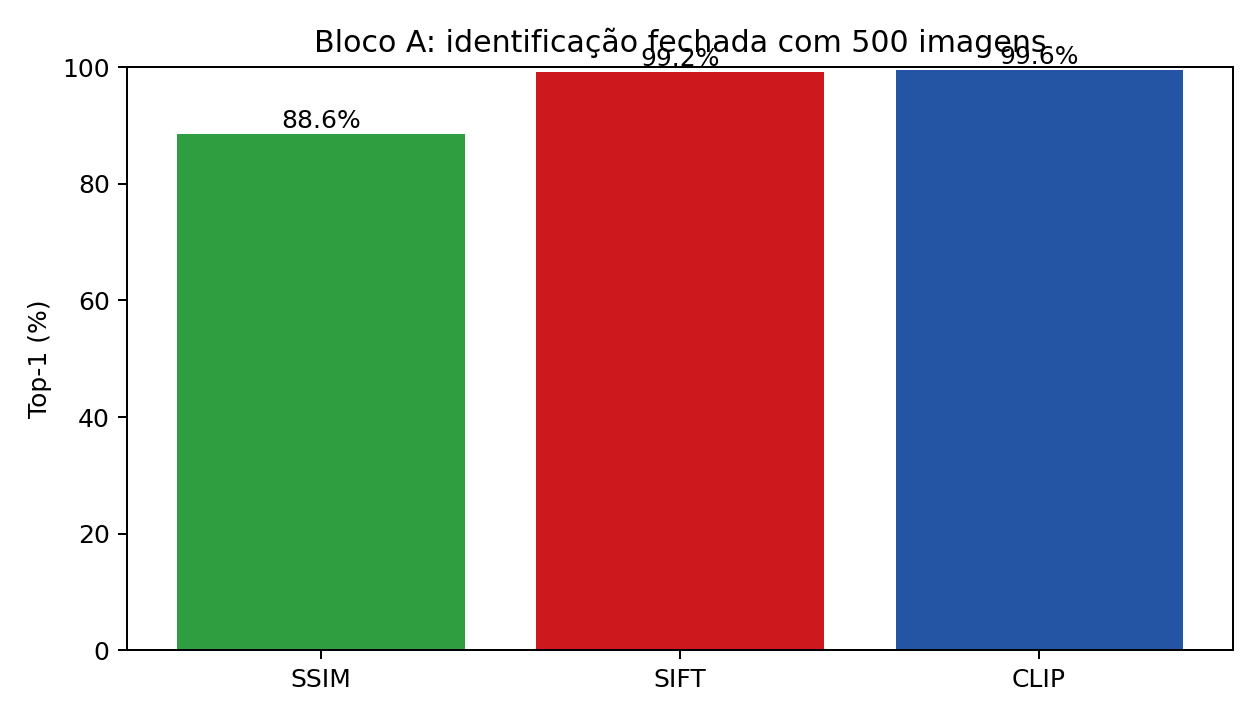
\includegraphics[width=0.82\textwidth]{results/pavd/block_a_top1.png}
\caption{Top-1 medido no Bloco A.}
\label{fig:block-a-top1}
\end{figure}

\begin{figure}[H]
\centering
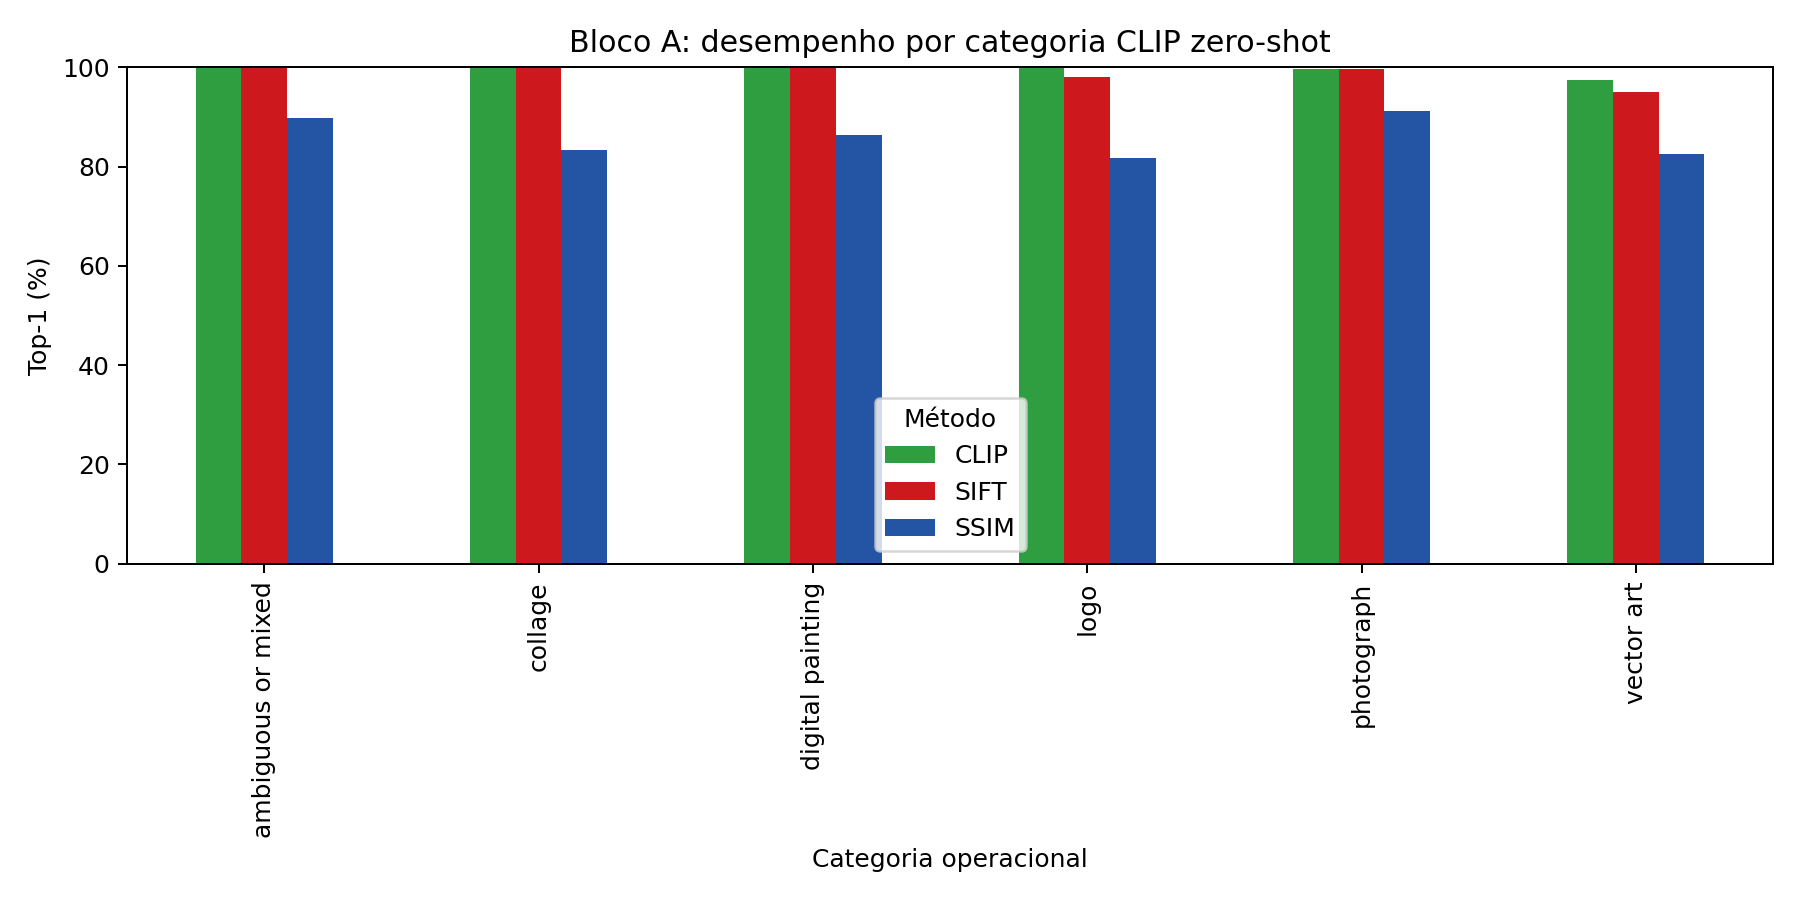
\includegraphics[width=\textwidth]{results/pavd/block_a_by_category.png}
\caption{Top-1 por categoria operacional estimada pelo CLIP.}
\label{fig:block-a-categories}
\end{figure}

\begin{table}[H]
\centering
\caption{Tabela gerada automaticamente para o desempenho por categoria.}
% Generated by python -m pavd.cli.build_tcc_report
\begin{tabular}{lrrrr}
\toprule
\textbf{Categoria} & \textbf{N} & \textbf{SSIM} & \textbf{SIFT} & \textbf{CLIP} \\
\midrule
ambiguous or mixed & 128 & 89.8\% & 100.0\% & 100.0\% \\
collage & 12 & 83.3\% & 100.0\% & 100.0\% \\
digital painting & 44 & 86.4\% & 100.0\% & 100.0\% \\
logo & 49 & 81.6\% & 98.0\% & 100.0\% \\
photograph & 227 & 91.2\% & 99.6\% & 99.6\% \\
vector art & 40 & 82.5\% & 95.0\% & 97.5\% \\
\bottomrule
\end{tabular}

\label{tab:block-a-categories-generated}
\end{table}

\section{Conclusão}

Este trabalho organizou o \pavd{} como um protocolo para localizar,
verificar, rejeitar e documentar potenciais correspondências visuais em
galerias derivadas de datasets web-scale. O Bloco A, já medido em uma galeria
de conveniência com 500 imagens, mostrou Top-1 de 88,6\% para \ssim{}, 99,2\%
para \sift{} e 99,6\% para \clip{} sob uma degradação fixa. Esses números são
úteis para comparar a configuração experimental local, mas não descrevem o
LAION em geral.

Os blocos de galeria expandida, reranking híbrido e conjunto aberto foram
formulados para permitir uma avaliação posterior de escala, custo, impostores
semânticos e falsa atribuição. Seus resultados devem ser preenchidos somente
com medições auditáveis. Em qualquer escala, a correspondência visual deve
ser interpretada como evidência técnica reproduzível para auditoria, revisão
humana e eventual análise especializada, e não como prova jurídica conclusiva.

\bibliographystyle{sbc}
\bibliography{referencias}

\end{document}
